\section{Problem}

The Medical test Records project approaches two main issues that hospital information systems face. \\

The first issue, is controlling access to a patient's profile.
A patient's profile has associated with it a group of information with different levels of sensitivity, such as age, name, blood type, diseases, family records and others.
A patient's name is not extremely sensitive so most employees can access it. However, for instance,the patient's family records do not need to be accessed nor should be accessible to most of the hospital staff, for example to volunteers. \\

Given this scenario, the access control mechanism must be able to correctly determine, and enforce the correct policies so that different parts of a patient's profile are only available to whom actually requires them to fulfill one's obligations to the patient, regarding the performed role and in the correct context. \\

The second problem comes from medical tests being analyzed in different facilities, like partner labs, that are not part of the hospital infrastructure, but require that both are interconnected in a way that enables all sides to identify each other and communicate in a secure way. \\

\subsection{Requisites}

Given the previous problems, the implementation of this project requires the following security guarantees:
\begin{itemize}
	\item A fine grained access control and secure authentication mechanism.
	\item Authenticity of all communications with the information systems.
	\item Confidentiality of all communications with the information systems.
	\item Integrity of all communications with the information systems.
	\item Non-repudiation of the communications with the partner labs.
\end{itemize}

\subsection{Trust assumptions}


There are three main entities in this project:\\
\begin{itemize}
	\item The Hospital System
		\subitem The system that will store all the patient data and tests results received from the labs.
	\item The Partner Labs System
		\subitem The partner lab can be internal, or external to the Hospital network. The internal lab is in the same network as the Hospital, but as the external lab, they will have different infrastructures from the hospital, which means they will have their own certificates and machines.
	\item The users of those systems, the staff.
	\item The certificate authority.
\end{itemize}


In case of the staff there is a full trust assumption that they won't have their credentials stolen, shared or compromised in any way, and as such we will not provide any mechanism to rapidly revoke those credentials. \\

Regarding the certificate authority, there is a full trust assumption that the private key used to issue/sign certificates won't be stolen and as such, we won't have a mechanism to revoke certificates. \\

Concerning the access control components which will be explained further (PDP,PEP...), there is a full trust assumption that those components will be correctly and logically well implemented, and won't allow any type of unauthorized access, but at the same time correctly serving good requests. \\

All communications with the partner labs (internal or external) will use HTTP requests with a custom security protocol, and will be considered secure and resistant against attacks like replay, tampering and eavesdropping. \\

There is also a full trust assumption, that all the libraries and frameworks used are error free and won't give any type of access to an attacker. \\


\section{Proposed solution}

\subsection{Overview}

The implementation will be separated in three API's, an hospital API, a laboratory REST API and an Access Control REST API, all developed using the framework Spring MVC\cite{springmvc}.

All the components involved in this project, will be developed using the Java\cite{java} programming language. \\

All requests received by the Hospital API will be intercepted by an access control mechanism and redirected to the access control API for validation. This access control API, for requests like getting a patient treatment will require a group of extra information to determine if the requests should be permitted or denied (e.g. role of the person making the request).
This set of information is added to the access control request by the Hospital API based on the presence (or lack of) of a token, this token is provided by the Hospital API on authentication to an end-user (e.g. Doctor) if the correct set of credentials (username:password) were supplied during the "login" action. The token is transported in the "Authorization" header of the HTTP request from the end-user to the Hospital API. In reality the Hospital API, for optimization, will know that if the request is not to the "login" action and doesn't posess a token, the PDP will never PERMIT the action to continue, so it denies the request before interrogating the PDP for authorization, to avoid a useless trip. \\

The database will store the hash version of the password using the Bcrypt\cite{bcrypt} algorithm, which already salts the passwords and avoids rainbow table attacks. The API will use a set of methods already provided by the spring-security-crypto\cite{springsecuritycrypto} module to validate the received credentials by hashing them and comparing to the value already stored in the database. BCrypt provides a set of mechanisms that allows to increase the complexity of the algorithm to use, to increase the time of processing and delay brute-force attacks. This complexity can be increased with time to adapt to the evolution of processing power on computers. \\


\\
The access control mechanism is composed by 4 components:
\begin{itemize}
	\item PEP - Policy Enforcement Point
	\item PDP - Policy Decision Point
	\item PAP - Policy Administration Point
	\item Policy Store
\end{itemize}

The PEP will send a XACML\cite{xacml} request to the PDP, the PDP will then based on the policies defined by the system return a XACML response which will dictate the action (ACCEPT or REFUSE) that PEP will enforce. If the result is ACCEPT, the request will continue and read or write the requested resource, otherwise the request will be dropped and replied with a 403 UNAUTHORIZED.

	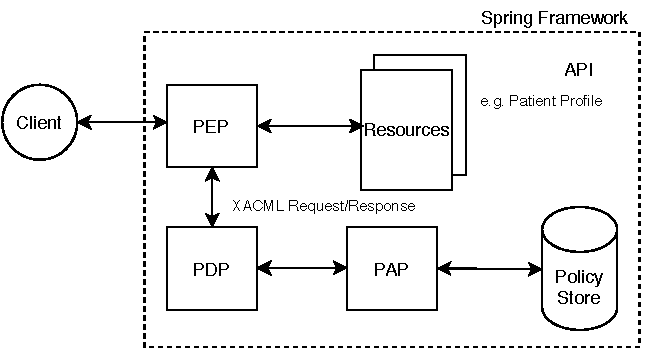
\includegraphics[width=.6\textwidth]{figs/access_control.pdf}


The PEP will be contained on the Hospital API and the rest of the components will be part of the Access Control API, this way the access control mechanism is externalized providing a more robust security in case the Hospital API gets somehow compromised. \\

\subsection{Deployment}
The following figure includes the distinct machines of this system, and as mentioned they will be interconnected through secure channels (TLS or custom protocol).

	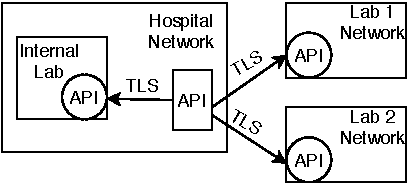
\includegraphics[width=.4\textwidth]{figs/infrastructure.pdf}

A staff member of the hospital , for example a doctor, will start by sending a request to the Hospital API requesting the test results of a given patient. The Hospital API will then make a request to the Lab API requesting the actual test results data.

The deployment scripts will use Vagrant\cite{vagrant} to manage and deploy the VM's and Ansible\cite{Ansible} for infrastructure providing (POSTGRESQL, JDK, CA installation...). \\

In this project there will be used only one external lab, but thats only for ease of management, as adding more lab's is just a matter of editing the deployment scripts. Also, in the diagram where there is an API circle, there are actually two machines, one with the Hospital API which contains the PEP and the other with the rest of the access control components (PDP,PAP...), as explained previously.


\subsection{Secure Channels}

All communications between the end-users (staff) and respective API's will run with TLS to provide confidentiality, integrity and freshness. TLS, between those entities will be provided by the Spring framework\cite{springmvc}, which is the framework and language that will be used to develop the project. As Spring default cipher suites already use by default the key exchange algorithm Diffie-Hellman, we won't override this configuration, as we want the Perfect Forward Secrecy property that comes from it.  \\

The communications between the Hospital API and partner lab API will be under a custom made protocol which will provide the same properties as a TLS channel (confidentiality, integrity and freshness). \\
	
The secure channels will require the definition of a certificate for each entity, we will consider that the certificates are installed manually by an administrator (during the provisioning process) on each respective machine.
We will have a made-up CA, which we will use to issue and sign the hospital, lab and access control API's certificates (including labs inside the hospital)(certificates created with OpenSSL\cite{openssl}). Those certificates alongside with the secure communication channel, will be used to digitally sign the sent tests data to guarantee its authenticity at any time.
In order to validate the certificates received by each API during the TLS Handshake, each machine will have the root CA certificate already installed, manually, by an administrator (again, during the provisioning process).\\ 
 
\subsection{Secure Protocol to Develop}
The custom protocol to develop, will enable secure communications between the Hospital API and partner lab, providing the same properties as TLS.
This protocol will work on top of the HTTP protocol and not under it like TLS, this means that the handshakes, message exchanges will all happen with HTTP requests.

In our case we will only support one cipher suite, the protocols to be used will be RSA for key exchanging, AES-256 for block cipher and hmac-sha256 for message authentication.

When a doctor makes a test data request, the Hospital API will be in charge of starting the handshake with the Lab API, by making a request to a special endpoint with its certificate before exchanging any data.  After the lab receives the certificate, it will verify it by checking its hostname (to see if its actually a valid person in the hospital side making the request), expiration date and validity with the CA. If it's all ok, the client will generate a pseudo-random secret (random byte string), encrypt it with the receiver/target public key and send that ciphered value back. From that secret, both Hospital (the hospital obtains the random string by decrypting it with it's own private key) and Lab API's will generate session keys. Finished this handshake, the hospital will now make a request to the lab API encrypting the request with the session key and adding a TAG (for integrity) using the same session key, for more security the key shouldn't be the same, but we will leave that to the advanced version if there is time. The Lab will then will answer with the test results data encrypted and protected using the same generated session key. Finally, all the messages will also have an NONCE to protect from message replay. \\


\section{Results}

From the basic functionalities described in the API (docs/API.md) documentation file, all the endpoints were implemented and their data access layer concluded. Given that, is possible to make requests to a patient name, diseases, treatment... without any kind of limitation or access control, with that in mind the access control mechanisms and API were implemented next. \\

As previously described this mechanism is structured into different interception points (Policy Enforcement Point, Policy Decision Point and Policy Administration Point), the PDP and PAP were implemented in the PDP/Access Control API, successfuly externalizing the policies in another place. The PEP was also successfully implemented in the Hospital API and communicating in a secure way with the rest of the externalized components using the XACML framework rules, inspired by the Authz framework\cite{authz}.

\subsection{Basic}
\begin{itemize}
	\item API.
		\subitem The following endpoints will exist in the API:
		\subitem - GET /patient/{id}/name, returns the name of the patient with id {id}.
		\subitem - GET /patient/{id}/diseases, returns the diseases the patient has (e.g. tuberculosis...)
		\subitem - GET /patient/{id}/treatment, the necessary treatment (e.g. what medicine the patient needs, 500mg of Vicodin).
		\subitem - GET /patient/{id}/testsresults, the results of the tests.
		\subitem - POST /testresults/{id}, used by the partner labs to write the tests results.
	\item TLS for secure communication channels with the end-users.
	\item Access Control.
		\subitem The following roles will exist: Doctor, Nurse, Janitor and Lab Employee. The doctor role will give read access to any information about the patient, the nurse role will give read access to any information regarding the necessary treatment (e.g. food, medicine...), the janitor role will only give  read access to superficial information like the patient name, finally the lab employee won't have access to any patient profile information, they can only see in their entity respective API if there is any requests from the hospital to process tests data and writing the results of the tests data.
	\item Custom communications protocol. (Hospital - Partner lab's).
\end{itemize}

It is expected that this version will take around 2 weeks to complete. 


\subsection{Intermediate}
\begin{itemize}
	\item The necessary mechanism to check tests data authenticity at any time. (Digital Signature)
	\item Sensitive information like passwords stored in a safe way using Bcrypt (already salts).
	\item Finishing the implementation of the custom communications protocol
\end{itemize}

This phase should take around 2 week's.


\subsection{Advanced}
\begin{itemize}
	\item Encryption of all the confidential information in the database, to avoid leaks in case of a breach.
	\item Policies and authentication information cache. (Will avoid constant reads to the database everytime there is a request).
	\item Defining rule combining algorithms in the access control for  more complex decisions.
	\item Firewall implementation.
	\item Maximum number of login attempts.
	\item Finished message improved to avoid tampering during the custom protocol handshake.
\end{itemize}


\subsection{Effort Commitment}

\begin{tabularx}{0.8\textwidth} { 
  | >{\centering\arraybackslash}X 
  | >{\centering\arraybackslash}X 
  | >{\centering\arraybackslash}X 
  | >{\centering\arraybackslash}X | }
 \hline
  & Alexandru & Ana Marta & Rafaela \\
 \hline
 Week 1  & API & Deployment Scripts & Database \\
  \hline
  Week 2  & Access Control  & Custom Protocol & Tests data authenticity mechanism \\
   \hline
   Week 3  & Access Control  & Custom Protocol  & Tests data authenticity mechanism \\
    \hline
    Week 4  & Firewall  & Rule Combining Algorithms  & Database encryption \\
\hline
\end{tabularx}


\begin{thebibliography}{9}
\bibitem{springmvc} 
Pivotal Software, Spring MVC
\\\texttt{https://docs.spring.io/spring-framework/docs/3.2.x/spring-framework-reference/html/mvc.html}

\bibitem{bcrypt} 
Niels Provos and David Mazières, bcrypt
\\\texttt{https://auth0.com/blog/hashing-in-action-understanding-bcrypt}

\bibitem{xacml} 
OASIS, XACML
\\\texttt{https://www.oasis-open.org}

\bibitem{vagrant} 
HashiCorp, Vagrant
\\\texttt{https://www.vagrantup.com/}

\bibitem{openssl} 
The OpenSSL Project, OpenSSL
\\\texttt{https://www.openssl.org/}

\bibitem{java} 
Oracle, Java
\\\texttt{https://java.com/}


\end{thebibliography}

